\section{Deep Convolutional Neural Network}
\label{sec:cnn}

This chapter serves as an introduction to the basic notions that will come up in the remaining of this thesis, namely the notion of Deep Neural Network (NN) and Deep Convolutional Neural Network (CNN).
We start by introducing generalities about neural networks.
Most of the content of the present chapter is taken from \cite{goodfellow16}

\subsection{Neural Network}
Deep learning essentially refers to a family of machine learning methods that historically derive from the multilayer perceptron (MLP), also known as Neural Network.
An MLP aims at approximating a function $f^{*}$ with a function $f(x;\theta)$ parameterized by $\theta$.
More concretely, an MLP converts an input $x$ to an output $y$ using a chain of function $f^{(1)} \circ f^{2} \circ \cdots \circ f^{n}(x)$, which justifies its name ``network''.
Each function is usually referred to as ``layer'', while the term ``neural'' comes from the fact that it is originally inspired by neuroscience \cite{mcculloch43}.

As in all machine learning setup, one wants to find the set of parameters $\bm{\theta}$ so as to optimize a cost function, for example the Mean Squared Error (MSE):

\begin{equation}
\mathcal{L}(\bm{theta}) = \sum_{x\in \mathcal{X}}(f^{*}(x)-f(x;\bm{\theta}))
\end{equation}

One typically use a gradient-descent method to solve the above problem.

In the frame of MLP, the functions $f^{m}(x;\bm{\theta_{m}})$ are linear (or fully-connected) layer, i.e. $\bm{theta}_m=(\bm{w)_{m},b$, followed by an activation function $\sigma(.)$

\begin{equation}
f^{m}(x;\bm{\theta_{m}}) = \sigma(\bm{x}^{T}\bm{w} + b)
\end{equation}

The activation function, allows to inject non-linearities in the model.
Such function is applied element-wise.
The rectifier liner unit (ReLU) is the most widespread.
It writes:

\begin{equation}
\sigma(x) = \max \{0, \bm{x}\}
\end{equation}

\subsection{Convolutional Network}
Many machine learning applications relie on structured data, i.e. data that respect a grid-like topology.
Typical examples include time-series and images.
For this reason, \cite{lecun95} introduced the notion of convolutional network, which adapts the previous MLP to leverage the grid-like topolgy in an effective manner.
In particular, the author replaces one or several layers of an MLP with convolutional layers.
In the case of (discrete) images, the convolution operator writes:

\begin{equation}
S(i,j) = (I * K)(i,j) = \sum_{m} \sum_{n} I(m,n) K(i-m, j-n)
\end{equation}

where $I$ is a grayscale image and $K$ is a kernel.
This formulation naturally extends to multi-channel images.
The convolutional operator brings the following advantage over the MLP: (1) It naturally leverages the spatial connectivity of pixels.
(2) As the size of the kernel is usually much smaller than the input size (sparse-connectivity), the number of parameters are greatly reduced, which reduces the memory consumption, accelerates the training and improves performances \cite{lecun95}.
Fig. \ref{fig:cnn_con} illustrates the idea of sparse connectivity brought by convolutional layers.

\begin{figure}[!htpb]
  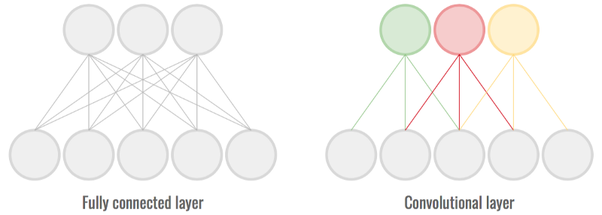
\includegraphics[width=13cm]{theory/fc_vs_conv}
  \caption{(Left) A fully-connected (linear) layer with 1D input at the bottom. (Right) Convolutional layer with a kernel of size 3.}
  \label{fig:cnn_con}
\end{figure}

Another important component of Convolutional networks are pooling layers, which allow to increase the receptive field of the convolutional operators as the depth is increased.
This effectively allow to capture, in the case of images, visual features that at different spatial scales, i.e. more global as the depth increases.
In particular, the max-pooling operator computes for each spatial location the maximal filter response over a pre-defined neighborhood.
Figure \ref{fig:cnn} illustrates a CNN applied in the frame of an image processing task.

\begin{figure}[!htpb]
  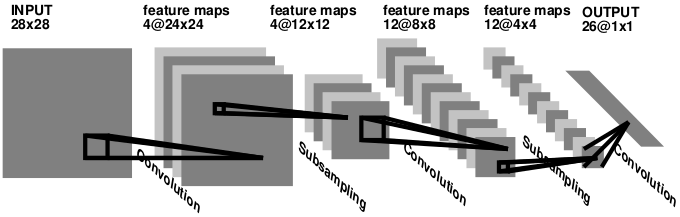
\includegraphics[width=13cm]{theory/cnn}
  \caption{Convolutional Neural Network applied to an image task.
    The network applies a succession of convolution, and pooling (subsampling) operation.
  Activation functions are not represented. Figure taken from \cite{lecun95}}
  \label{fig:cnn}
\end{figure}

%%% Local Variables:
%%% mode: latex
%%% TeX-master: "../../main"
%%% End:
